\documentclass[9pt]{beamer}
\usepackage[utf8]{inputenc}
\usepackage[russian]{babel}
\usepackage{graphicx, epsfig}
\usepackage{amsmath,mathrsfs,amsfonts,amssymb}
\usepackage{subfig}
\usepackage{floatflt}
\usepackage{epic,ecltree}
\usepackage{mathtext}
\usepackage{fancybox}
\usepackage{fancyhdr}
\usepackage{multirow}
\usepackage{enumerate}
\usepackage{epstopdf}
\usepackage{multicol}
\usepackage{algorithm}
\usepackage[noend]{algorithmic}
\def\algorithmicrequire{\textbf{Input:}}
\def\algorithmicensure{\textbf{Output:}}
\usetheme{Singapore}%{Singapore}%{Warsaw}%{Warsaw}%{Darmstadt}
\usecolortheme{default}
\setbeamertemplate{footline}[page number]{}
\newcommand{\bx}{\mathbf{x}}
\newcommand{\by}{\mathbf{y}}
\newcommand{\bz}{\mathbf{z}}
\newcommand{\bw}{\mathbf{w}}
\newcommand{\ba}{\mathbf{a}}
\newcommand{\bb}{\mathbf{b}}
\newcommand{\bY}{\mathbf{Y}}
\newcommand{\bX}{\mathbf{X}}
\newcommand{\bu}{\mathbf{u}}
\newcommand{\bt}{\mathbf{t}}
\newcommand{\bp}{\mathbf{p}}
\newcommand{\bq}{\mathbf{q}}
\newcommand{\bc}{\mathbf{c}}
\newcommand{\bP}{\mathbf{P}}
\newcommand{\bT}{\mathbf{T}}
\newcommand{\bB}{\mathbf{B}}
\newcommand{\bQ}{\mathbf{Q}}
\newcommand{\bC}{\mathbf{C}}
\newcommand{\bE}{\mathbf{E}}
\newcommand{\bF}{\mathbf{F}}
\newcommand{\bU}{\mathbf{U}}
\newcommand{\bW}{\mathbf{W}}
\newcommand{\bM}{\mathbf{M}}
\newcommand{\bbR}{\mathbb{R}}
\newcommand{\cA}{\mathcal{A}}
\newcommand{\bchi}{\boldsymbol{\chi}}
\newcommand{\bnu}{\boldsymbol{\nu}}
\newcommand{\bmu}{\boldsymbol{\mu}}
\newcommand{\bOne}{\boldsymbol{1}}
\newcommand{\bZero}{\boldsymbol{0}}
\newcommand{\btheta}{\boldsymbol{\theta}}
\newcommand{\bTheta}{\boldsymbol{\Theta}}
\newcommand{\argmin}{\mathop{\arg \min}\limits}
\newcommand{\argmax}{\mathop{\arg \max}\limits}
\newcommand{\T}{\mathsf{T}}

\setbeamertemplate{navigation symbols}{}

\newcommand\undermat[2]{%
	\makebox[0pt][l]{$\smash{\underbrace{\phantom{%
					\begin{matrix}#2\end{matrix}}}_{\text{$#1$}}}$}#2}

\newtheorem{statement}{Утверждение}
\newtheorem{rustheorem}{Теорема}

% отображать название слайда слева
\setbeamertemplate{frametitle}[default][left]

\usepackage{tikz-cd}
%\definecolor{beamer@blendedblue}{RGB}{15,120,80}
%----------------------------------------------------------------------------------------------------------
\title[\hbox to 56mm{  \hfill\insertframenumber\,/\,\inserttotalframenumber}]
{\\ \vspace{1.5cm} Снижение размерности фазового пространства \\ в задачах канонического корреляционного анализа}
\author[Курдюкова Антонина]{\\ 
	\vspace{.4cm}
	Курдюкова Антонина\\
	\vspace{3mm}
	{\footnotesize Научный руководитель: \\
	д.ф.-м.н. В. В. Стрижов}}
\institute[МФТИ(НИУ)]{
Московский физико-технический институт\\
Факультет управления и прикладной математики\\
Кафедра <<Интеллектуальные системы>>}
\date{8 июня 2022 г.}
%--------------------------------------------------------------------------------
\begin{document}
%--------------------------------------------------------------------------------
\begin{frame}
%\thispagestyle{empty}
\titlepage
\end{frame}
%--------------------------------------------------------------------------------
\begin{frame}{Снижение размерности фазового пространства}
Решается задача декодирования сигналов. Требуется восстановить зависимость между двумя наборами гетерогенных данных.
	\begin{block}{Цель}
		Показать, что методы канонического корреляционного анализа являются частным случаем метода сходящихся перекрестных отображений Сугихары.
	\end{block}
	\begin{block}{Проблема}
		Сложная структура временного ряда -- наличие нелинейных зависимостей и варьирующийся период. 
		\vspace{0.5cm}
		
		Требуется построить адекватрную модель прогноза сигнала гироскопа по сигналу акселерометра для ходьбы.
	\end{block}
	\vspace{-0.2cm}
	\begin{block}{Решение}
		 Предлагается использовать скрытое пространство, снизив размерность исходного фазового пространства, и применить метод сходящихся перекрестных отображений для учёта причинно-следственных связей между временными рядами. 
	\end{block}
\end{frame}
%--------------------------------------------------------------------------------
\begin{frame}{Литература}
\begin{block}
 {Предлагается латентный CCM для выявления причинно-следственных связей в хаотических динамических системах}
\begin{itemize}
		\item De Brouwer E. et al. Latent convergent cross mapping //International Conference on Learning Representations, 2020
	\end{itemize}
\end{block}
% \begin{block}{Решается задача аппроксимации фазовой траектории, построенной по квазипериодисческому временному ряду }
% \begin{itemize}
% 		\item Усманова К. Р. и др. Аппроксимация фазовой траектории квазипериодических сигналов методом сферической регрессии // Вычислительная математика и кибернетика, 2020
% 	\end{itemize}
% \end{block}
\begin{block}{Предложены методы декодирования сигналов. Учитываются зависимости в исходном и целевом пространствах, а также случай избыточности описания исходных данных}
 	\begin{itemize}
		\item Исаченко Р. В., Стрижов В. В. Снижение размерности пространства в задачах декодирования сигналов, 2018
	    
	\end{itemize}
\end{block}
\begin{block}{Предлагаемый метод осуществляет нелинейную реконструкцию пространства состояний по временному ряду и позволяет отличить причинность от корреляции во временных рядах}
\begin{itemize}
		\item Sugihara G. et al. Detecting causality in complex ecosystems //Science, 2012
	\end{itemize}
\end{block}
	
\end{frame}
%--------------------------------------------------------------------------------
\begin{frame}{Прогностическая модель в задаче декодирования}
\begin{columns}
\column{.4\textwidth}
\begin{block}{Дано}
	\vspace{0.1cm}
	Выборка -- $\left( \bx, \by \right)$,\; где \quad
	$\bx = \{ x_1,\dots, x_{N_1}\}$,\quad
	$\by = \{ y_1,\dots, y_{N_2}\}$.\\
	\vspace{0.3cm}
	Требуется построить прогноз ряда $\by$ на $m$ значений вперед:   \[y_{N_2 + 1},\dots, y_{N_2 + m}.\]
	При построении прогноза учесть влияние ряда $\bx$ на $\by$.
	\end{block}
\vspace{0.3cm}
\column{.6\textwidth}
\includegraphics[width=6cm]{Slides/images_pr/acc+gyr.png}
\end{columns} 
\vspace{-0.2cm}
\begin{block}{Прогноз на один шаг вперед}
    \vspace{-0.1cm}
	\[
		\hat{y}_{t+1} = \mathcal{F}(\hat{\bw}, y_t,\dots,y_{t-h+1}, x_t,\dots,x_1),
	\]
	\[
	    \hat{\bw} = \arg\min_{\bw} \mathcal{L}(\bw, \bx, \hat{\bx}),
	\]
	здесь $\mathcal{L}$~-- функция потерь, $h$~---горизонт прогнозирования.
\end{block}	
	

	
\end{frame}
%--------------------------------------------------------------------------------
\begin{frame}{Построение фазового пространства}
\vspace{0.3cm}
Траекторная матрица временного ряда $\bx$\\
Точки $\bx_j\in\mathbb{R}^k$\; образуют фазовую траекторию
\vspace{0.2cm}
        \[ \mbox{\bfseries X} = \begin{bmatrix}
                        x_1 & \dots & x_k \\
                        x_2 & \dots & x_{k+1} \\
                        \hdotsfor{3} \\
                        x_{n} & \dots & x_{N_1}
                        \end{bmatrix}^{\mathsf{T}} = \begin{bmatrix} \bx_1 & \dots & \bx_{n} \end{bmatrix},\]
\vspace{0.1cm}
где $k$ - ожидаемая длина периода, $n = N_1 - k + 1$.                        
\hfil\hfil\includegraphics[width=4.5cm]{Slides/images_pr/ts_slide_new.png}
\hfil\hfil\includegraphics[width=5cm]{Slides/images_pr/st2_new.png}


\end{frame}
%--------------------------------------------------------------------------------
\begin{frame}{Аттрактор Лоренца}
Динамическую систему можно описывать системой дифференциальных уравнений:
$$
    \begin{cases}
        \dot X = \sigma(Y -X)\\
        \dot Y = X(r - Z) - Y\\
        \dot Z = XY - bZ,
    \end{cases}
$$
где $\sigma, \, r,\, b$~--- параметры.

\vspace{0.3cm}
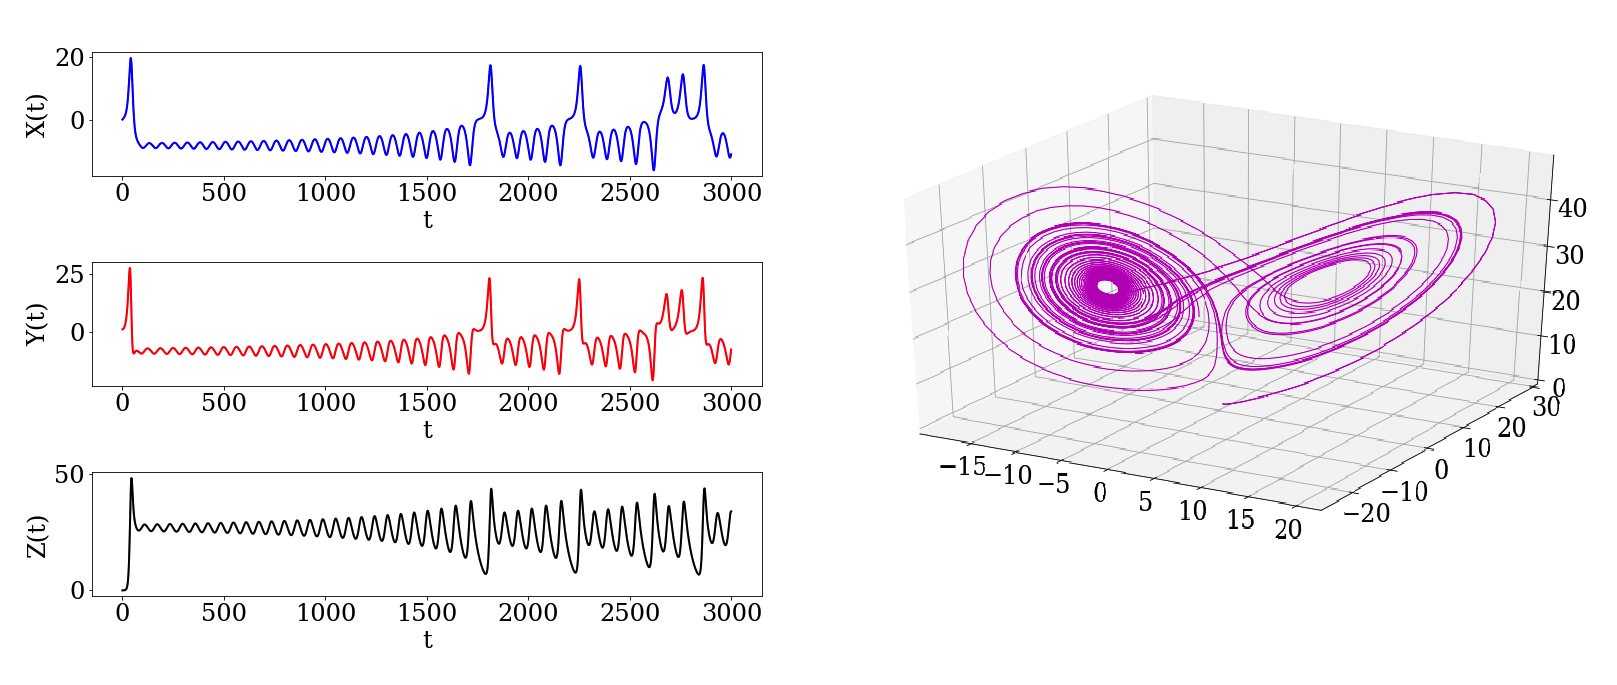
\includegraphics[width=11cm]{Slides/images_pr/ts_xyz.png}

\end{frame}
%--------------------------------------------------------------------------------
\begin{frame}{Теорема Такенса о вложениях}
\vspace{0.2cm}
Теорема формулирует условия, при которых аттрактор динамической системы можно восстановить по временному ряду лишь одной из наблюдаемых.\\
Диффеоморфизм $\phi(x)$ отображает аттрактор $\bM$ в его скрытое представление~$\bM_X$:
\[ \phi(x) = (\alpha(x),\, \alpha(f_M(x)),\, \dots,\, \alpha(f_M^{d-1}(x))),\]
где $\alpha:\: \bM\rightarrow \mathbb{R}$~--- функция наблюдений, $f_M$ задает динамику системы, $d$~--- размерность скрытого представления.

\vspace{0.2cm}
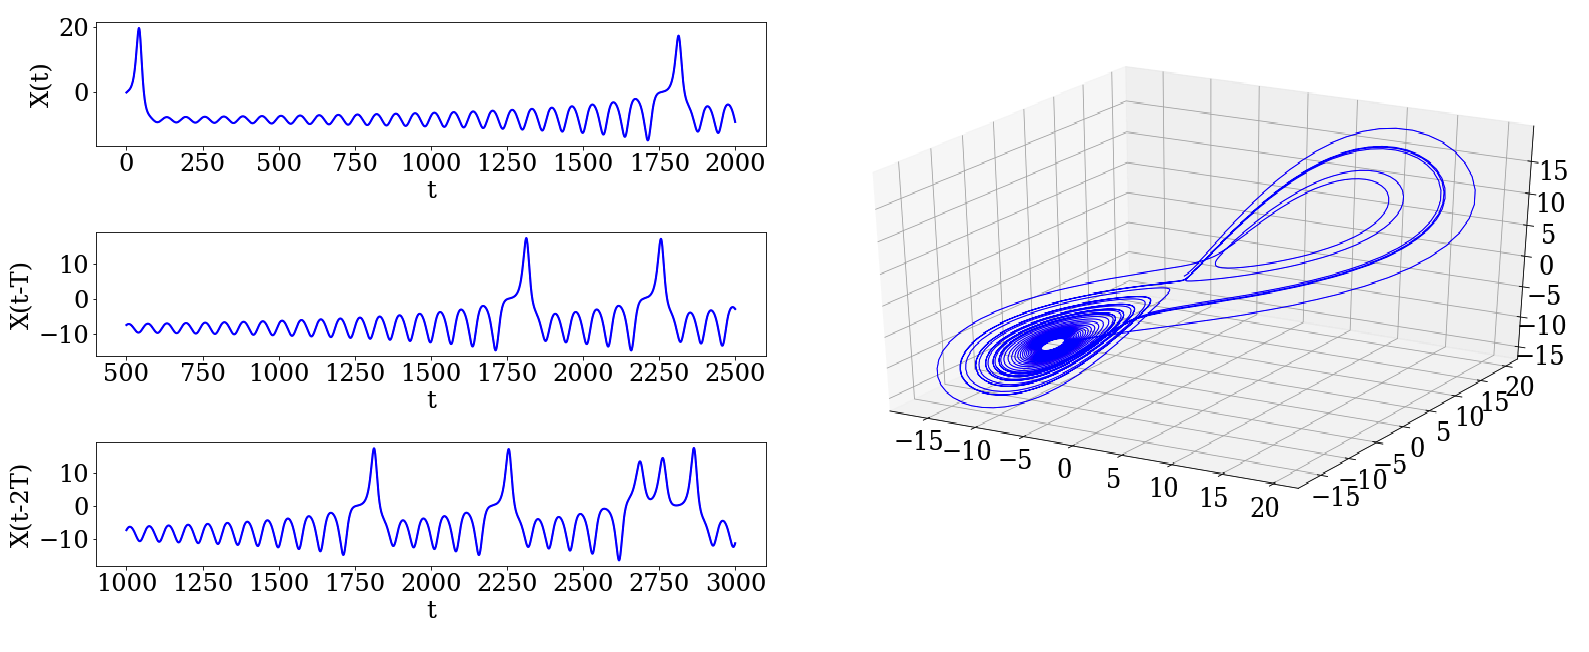
\includegraphics[width=11cm]{Slides/images_pr/attractor_X.png}

\end{frame}
%--------------------------------------------------------------------------------

\begin{frame}{Метод перекрестных сходящихся отображений}
\vspace{0.25cm}
Выберем точку фазовой траектории $\bx_0\in\bX$.\\
Найдем $k$ ближайших соседей $\bx_{t_1},\dots, \bx_{t_k}\in \bX$.\\
Временным индексам $t_1,\dots,t_k$ соответствуют точки $\by_{t_1},\dots, \by_{t_k}\in\bY$.
\vspace{0.2cm}
\begin{block}{Введем отображение:}
\vspace{-0.2cm}
\[ \varphi: \bx_0 \mapsto \widehat{\by_0} = \sum\limits_{i=1}^k w_i \by_{t_i}, \qquad 
w_i = \dfrac{u_i}{\sum\limits_{j=1}^k u_j}, \qquad
u_i = \exp \bigl( -||\bx_0 - \bx_{t_i}|| \bigr).\]
\end{block}
\vspace{-0.2cm}
\begin{figure}[h]
\centering
\includegraphics[width = 290]{Slides/images_pr/knn.png}
\end{figure}

\end{frame}
%--------------------------------------------------------------------------------
\begin{frame}{Зависимость между временными рядами}
\vspace{-0.5cm}
\begin{columns}
\column{.5\textwidth}
\begin{block}{Липшицевость отображения}
Временные ряды $\bx$ и $\by$ называются \textbf{связанными}, если отображение $\varphi$ является липшицевым:
	$$ \rho_{\bY}(\varphi(\bx_i), \varphi(\bx_j)) \leq C \rho_{\bX}(\bx_i, \bx_j), \quad \bx_i, \bx_j \in \bX. $$
\end{block}
\vspace{-0.4cm}
\begin{block}{Функция близости}
Для проверки наличия связанности введём метрическую функцию близости векторов в окрестностях $U_k(\bx_{0})$ и $U_k(\by_{0})$:
\end{block}
\column{.5\textwidth}
\begin{figure}[h]
\centering
\includegraphics[width = 170]{images_pr/CCM.jpeg}
\end{figure}
\end{columns}


\[
	L(\bx, \by) = \dfrac{R(U_k(\bx_{0}))}{R(U_k(\by_{0}))}, \qquad R(U_k(\bx_{0})) = \dfrac{1}{k} \sum\limits_{i=1}^k \rho_{\dH_{\bx}}(\bx_{0}, \bx_{t_j}).
\]

Если $L(\bx, \by)$ больше заданного порога, то временной ряд $\by$ зависит от временного ряда $\bx$.

%----------------------------------------------------------------------------------    
\end{frame}
\begin{frame}{Модель определения фазы}
\begin{columns}
\column{.45\textwidth}
  Модель $m: \varphi \rightarrow \mbox{\bfseries x}$ ставит в соответствие фазе $\varphi \in [0, 2\pi)$ точку ожидаемой траектории $\mathsf{E}(\hat{\mbox{\bfseries x}}|\varphi)$. 
\begin{block}{Регрессия Надарая-Ватсона}
\vspace{-0.3cm}
    \[ m(\varphi) = \mathsf{E}(\hat{\vec{x}}|\varphi) =\frac{\sum\limits_{\vec{x}\in \vec{X}}\vec{x'}K\left(\frac{\rho(\hat{\varphi} - \varphi)(\vec{x})}{h}\right)}{\sum\limits_{\vec{x}\in \vec{X}}K\left(\frac{\rho(\hat{\varphi} - \varphi)(\vec{x})}{h}\right)}.  \]
  \end{block}   
\vspace{-0.2cm}
\column{.55\textwidth}
\includegraphics[width=6cm]{Slides/images_pr/phas_final.png}
\end{columns} 
\vspace{-0.4cm}
\begin{block}{Функции потерь}
\vspace{-0.3cm}
\[L_1(\varphi) =
        \frac{1-\cos(\varphi-\varphi')}{2},\quad L_2(\varphi) = 
    \sum_{\| \mathbf{x} - \mathbf{x'} \|<\varepsilon, \; \mathbf{x'} \in \mathbf{X}}\rho( \varphi, \varphi'), \quad L_3(\varphi) = \frac{\|\mathbf{x} - m(\varphi)\|_2}{d(\varphi)}\]
\end{block}
\vspace{-0.4cm}
\begin{block}{Искомое значение фазы}
\vspace{0.1cm}
$\widehat{\varphi}_i = \arg\min_{\varphi} \lambda_1\cdot L_1(\varphi) + \lambda_2 \cdot L_2(\varphi) + \lambda_3 \cdot L_3(\varphi), \quad \sum_{i=1}^{3} \lambda_i = 1.$
    
\end{block}

\end{frame}
%--------------------------------------------------------------------------------
\begin{frame}{Снижение размерности фазового пространства}


\begin{block}{Линейная зависимость}
\vspace{0.1cm}
	$\bX\in\bbR^{k\times n},\, \bY\in\bbR^{k\times r}$~-- матрицы фазовых пространств $\bx,\,\by$.\\
	Предполагается линейная зависимость между строками $\bX$ и $\bY$:
	\[
	    \mathbf{Y}_i = \mathbf{X}_i\cdot\mathbf{\Theta} + \boldsymbol{\varepsilon} \quad \mathbf{Y}_i\in\bbR^r,\;\mathbf{X}_i\in\bbR^n,\; i = 1,\ldots,k.
	\]
\end{block}
\vspace{-0.3cm}
\begin{columns}
\column{.5\textwidth}
\begin{block}{Метод частичных наименьших квадратов (PLS)}
	\vspace{-0.5cm}
\begin{align*}
\underset{k \times n}{\vphantom{\bQ}\bX} 
&= \underset{k \times l}{\vphantom{\bQ}\bT} \cdot \underset{l \times n}{\vphantom{\bQ}\bP^{\T}} + \underset{k \times n}{\vphantom{\bQ}\bF} 
= \sum_{j=1}^l \underset{k \times 1}{\vphantom{\bp_j^{\T}}\bt_j} \cdot \underset{1 \times n}{\bp_j^{\T}} + \underset{k \times n}{\vphantom{\bp_j^{\T}}\bF}\\
\underset{k \times r}{\vphantom{\bQ}\bY} 
&= \underset{k \times l}{\vphantom{\bQ}\bU} \cdot \underset{l \times r}{\bQ^{\T}} + \underset{k \times r}{\vphantom{\bQ}\bE}
=  \sum_{j=1}^l  \underset{k \times 1}{\vphantom{\bq_j^{\T}}\bu_j} \cdot \underset{1 \times r}{\bq_j^{\T}} +  \underset{k\times r}{\vphantom{\bq_j^{\T}}\bE}
\end{align*}
\end{block}
\column{.5\textwidth}

\[
        \begin{tikzpicture}
			\matrix (m) [matrix of math nodes,row sep=3em,column sep=1em,minimum width=2em,ampersand replacement=\&]
			{
			    \& S \&
			    \\
				\mathbf{X}\in\bbR^{k\times n} \& \& \mathbf{Y}\in\bbR^{k\times r} \\
				\& \mathbf{T}, \mathbf{U} \in \bbR^{k\times\ell} \& \\};
			\path[-stealth]
			(m-1-2) edge [bend right=10] node {} (m-2-1)
			(m-1-2) edge [bend left=10] node {} (m-2-3)
			(m-2-1) edge node [above] {$\mathcal{F}$} (m-2-3)
			(m-2-1) edge [bend right=10] node [below, pos=0.4] {} (m-3-2)
			(m-3-2) edge [bend right=10] node [above, pos=0.4] {$\bP$} (m-2-1)
			(m-2-3) edge [bend left=10] node [below, pos=0.4] {} (m-3-2)
			(m-3-2) edge [bend left=10] node [above, pos=0.4] {$\bQ$} (m-2-3);
		\end{tikzpicture}
    \]
\end{columns}
\vspace{-0.5cm}
\begin{block}{Ошибка}
	\vspace{-0.2cm}
\[
    L(\mathbf{\Theta}, \mathbf{X}, \mathbf{Y}) = \|\mathbf{Y} - \mathbf{X}\cdot\mathbf{\Theta}\|_2^2
\]
\vspace{-0.2cm}
\[
    \mathbf{\Theta} = \mathbf{W}(\mathbf{P}^{\mathsf{T}}\mathbf{W})^{-1}\mathbf{Q}^{\mathsf{T}}
\]
\end{block}
\end{frame}
%--------------------------------------------------------------------------------
\begin{frame}{Вычислительный эксперимент}
\begin{block}{Данные}
\vspace{0.3cm}
\hfil\includegraphics[width=6.5cm]{images_pr/signal.png}
\hfil\includegraphics[width=4cm]{images_pr/gyr_tr.png}
\end{block}
\begin{block}{Ошибка предсказания алгоритма PLS}
\vspace{-0.3cm}
\begin{table}[bhtp]
	\centering
	\label{tbl:methods}
	\begin{tabular}{l|l|l|l|c}
		\hline
		& Датчики & Прибор & Тип движения & MSE \\
		\hline
	1 & Акселерометр + гироскоп & один & ходьба & 0.006 \\
	2 & Акселерометр + гироскоп & один & медленная ходьба & 0.069  \\
	3 &	Акселерометр + акселерометр & разные & ходьба & 0.997  \\
	4 &	Акселерометр + гироскоп & один & бег & 0.027  \\
	5 &	Акселерометр + гироспкоп & один & быстрая ходьба & 0.024  \\

		\hline   
	\end{tabular}
\end{table}
\end{block}

\end{frame}

%--------------------------------------------------------------------------------
\begin{frame}
% 0.664+-0.01  0.411+-0.33  0.108+-0.13  0.596+-0.02  0.029+-0.14
% 0.663+-0.01  0.409+-0.28  0.077+-0.08  0.581+-0.03  0.017+-0.15
% Коэффициент корреляции Пирсона между истинным и предсказанным сигналами
% \vspace{-0.5cm}
% \begin{table}[bhtp]
% 	\centering
% 	\label{tbl:methods}
% 	\begin{tabular}{l|l|l|l|l|l|l|l|l|l|c}
% 		\hline
% 	      & 1 & 2 &  3 &  4 & 5 &  6 &  7 & 8 &  9 & 10 \\
% 		\hline
% 	    1 & 0.77 & 0.80 & 0.73 & 0.63 & 0.70 & 0.88 & 0.67 & 0.70 & 0.76 & 0.62 \\
% 		2 & -0.23 & 0.92 & 0.74 & -0.12  & 0.71 & 0.89 & 0.92 & 0.91 & -0.24 & -0.39  \\
% 		3 & 0.32 & 0.10 & 0.03 & -0.10 & -0.17 & 0.20 & 0.65 & -0.66 & 0.34 & 0.37 \\
% 		4 & 0.80 & 0.75 & 0.66 & 0.50 & 0.48 & 0.47 & 0.71 & 0.68 & 0.54 & 0.37  \\
% 		5 & -0.05 & 0.53 & -0.04 & -0.44 & 0.27 & -0.18 & -0.24 & -0.30 & -0.10 & 0.74  \\
% 		\hline   
% 	\end{tabular}
% \end{table}
% \vspace{0.5cm}
% Коэффициент корреляции Спирмена между истинным и предсказанным сигналами
% \vspace{-0.5cm}
% \begin{table}[bhtp]
% 	\centering
% 	\label{tbl:methods}
% 	\begin{tabular}{l|l|l|l|l|l|l|l|l|l|c}
% 		\hline
% 	      & 1 & 2 &  3 &  4 & 5 &  6 &  7 & 8 &  9 & 10 \\
% 		\hline
% 	    1 & 0.74 & 0.77 & 0.71 & 0.51 & 0.64 & 0.83 & 0.60 & 0.51 & 0.69 & 0.63 \\
% 		2 & -0.24 & 0.90 & 0.66 & -0.16  & 0.74 & 0.83 & 0.86 & 0.89 & -0.02 & -0.37  \\
% 		3 & 0.31 & 0.13 & -0.10 & -0.11 & -0.11 & 0.21 & 0.45 & -0.51 & 0.30 & 0.09 \\
% 		4 & 0.81 & 0.78 & 0.51 & 0.53 & 0.42 & 0.48 & 0.72 & 0.78 & 0.48 & 0.30  \\
% 		5 & 0.04 & 0.50 & -0.08 & -0.57 & 0.21 & -0.22 & -0.29 & -0.18 & 0.02 & 0.74  \\
% 		\hline   
% 	\end{tabular}
% \end{table}
\begin{block}{Корреляция Пирсона и Спирмена}
\vspace{0.05cm}
\begin{table}[bhtp]
	\centering
	\label{tbl:methods}
	\begin{tabular}{l|l|l|l|c}
		\hline
	      &  Прибор & Тип движения & $\mathsf{E}_p\pm\Variance_p$ & $\mathsf{E}_s\pm\Variance_s$  \\
		\hline
	1 &  Один & ходьба & $0.664\pm0.01$ & $0.663\pm0.01$        \\
	2 &  Один & медленная ходьба & $0.411\pm0.33$ & $0.409\pm0.28$  \\
	3 &	 Разные & ходьба & $0.108\pm0.13 $ & $0.077\pm0.08 $ \\
	4 &	 Один & бег & $0.596\pm0.02 $ & $0.581\pm0.03$  \\
	5 &	 Один & быстрая ходьба & $0.029\pm0.14$ & $0.017\pm0.15$  \\

		\hline   
	\end{tabular}
\end{table}
\end{block}
\vspace{-0.3cm}
\begin{block}{Зависимость ошибки MSE от величины сдвига сигналов}
\vspace{-0.05cm}
\includegraphics[width=10cm]{Slides/images_pr/delay.png}
\end{block}

\end{frame}
%--------------------------------------------------------------------------------

\begin{frame}{Выносится на защиту}
\begin{itemize}
	\item Исследовано утверждение о том, что методы канонического корреляционного анализа являются частным случаем метода перекрестных сходящихся отображений.
	\vfill
	\item Предложен метод обобщения PLS и CCM.
	\vfill
	\item Проведен вычислительный эксперимент на данных мобильного устройства.
	\vfill
	\item Показано, что учет зависимостей между временными рядами улучшает качество прогноза.
	\vfill
	\item Планируется рассмотреть другие методы канонического корреляционногот анализа.
\end{itemize}
\end{frame}
\end{document} 